%Packages are included below, these are akin to libraries in other programming languages. As far as I can tell, there is no reason to reduce the number of packages included in a document. It might compile faster, but overleaf compiles fast so this should not be an issue.
\documentclass[12pt,twoside]{report} %tells the compiler that this is a 'report' style document, and the main font size.
\usepackage{setspace} %allows the use of '\doublespace' to set line spacing
\usepackage[utf8]{inputenc} %inclusion of this is optional, overleaf includes it in its compiler so it is not necessary, it may be necessary for other compilers.
\usepackage[english]{babel} %this does a few things eg allowing dates to be made by the compiler. probably best not to get rid of it
\usepackage{wrapfig} %if it is desirable to wrap text (see https://www.overleaf.com/learn/latex/Wrapping_text_around_figures).
\usepackage{graphicx} %this allows graphics to be put in easily
\usepackage{float}%this allows you to put them in good places
\usepackage[version=4]{mhchem} %this is good for chemical reactions
\usepackage{amsmath} %maths package
\usepackage{amssymb} %symbol package
\usepackage{textcomp,gensymb} %more symbols (eg \degree)
\usepackage{appendix} %self explanatory
\usepackage{colortbl} %good for colouring in cells on a table
\usepackage{rotating} %allows you to rotate graphics
\usepackage{bm} %helps bold things
\usepackage{multirow} %for tables
\usepackage{longtable} %for long tables
\usepackage{booktabs} %more tables
\usepackage{pdfpages} %allows PDFs to be included in document (good if you want to include a pdf in an appendix eg)
\usepackage{caption} %allows captions for graphics
\usepackage[nottoc]{tocbibind} %adds the bibliography to the table of contents
\usepackage{subcaption} %allows subcaption for multiple images in one graphic

\PassOptionsToPackage{hyphens}{url}\usepackage{hyperref}
\usepackage{hyperref} %this is great for putting hyperreferences in the document.
\usepackage[table]{xcolor} %more colouring of tables
\definecolor{Gray}{gray}{0.9} %this defines a colour to be used and gives it a name. This is a colour called 'Gray' it is 'gray' with transparency 0.9
\hypersetup{colorlinks=false} %this stops links being colourful, which makes a report look less professional I believe.


\usepackage[letterpaper, top=0.5in, bottom = 0.5in, right = 0.5in, left=0.5in]{geometry} %this describes the layout of the document and the margins etc.
%\doublespacing %self explanatory
\renewcommand{\baselinestretch}{1.5}


\begin{document} % you have to do this to start the document

%%%%%%%%%%%%%%%%%%%%%%%%%%%%%%%%%%%%%%%%%%%
%For a long report such as a thesis, I would recommend thinking like programming, that is, have a short 'main' and long programs (or chapters in this case) this allows you to access each chapter easily and see the layout of the document easily.
%
%using \input{} basically puts the code specified in the argument (between the braces) into the body of the code in main
%%%%%%%%%%%%%%%%%%%%%%%%%%%%%%%%%%%%%%%%%%%

% The entire thesis is generated by the commands below, referencing the other files in this directory.

%%%%%%%%%%%%%%%%%%%%%%%%%%%%%%%%%%%%%%%%%%%
% Preamble
%%%%%%%%%%%%%%%%%%%%%%%%%%%%%%%%%%%%%%%%%%%

\begin{titlepage}
    \begin{center}
        \vspace*{2cm}
        % this title page can be played around with to better serve your project. the necessary parts to include are the TITLE at the top, the BLURB about the thesis presented etc. Name, faculty member, date, type of engineering...
        \LARGE
        \vspace{3cm}
        \textbf{Studying tissue-specificity of cancer in the context of \KRAS{}}

        \vfill
 
        \Large
        \textbf{Joshua H. Cook} \\
        \vspace{1cm}
        3rd year Ph.D. candidate \\
        Biological and Biomedical Sciences at Harvard Medical School \\
        email: jhcook@g.harvard.edu \\
        (Initial DAC meeting) \\
        Faculty Advisors: Kevin M. Haigis and Peter J. Park \\
        DAC Committee: Shamil Sunyaev (Chair), William Hahn, Matthew Meyerson \\
        June 10, 2020 from 3pm to 5pm \\
        The meeting will be held virtually over Zoom.\\
        \vspace{2cm}
 
    \end{center}
\end{titlepage}


\pagenumbering{roman} %Roman numbering is recommended until the body

\tableofcontents 

\listoffigures 

% \listoftables 

\chapter*{Abstract}
\normalsize

An abstract that provides a brief outline of the report.
 

\chapter*{Acknowledgements} %the star makes the chapter unnumbered
This is a good place to acknowledges those who helped you along the way. \\Also please note how LaTex has put this on a new page as it is a new chapter. No command (apart from starting a new chapter) was needed to do this. \\Also note the lack of number on the title, and contrast this to proceeding chapters, the abstract and acknowledgements should be unnumbered, the proceeding chapters should be numbered.

\pagenumbering{arabic} %back to Arabic numbering for the rest

%%%%%%%%%%%%%%%%%%%%%%%%%%%%%%%%%%%%%%%%%%%
% Chapters
%%%%%%%%%%%%%%%%%%%%%%%%%%%%%%%%%%%%%%%%%%%

\chapter{How to do Sections and Other Simple Text Formatting}
Here you should put a short introduction to your chapter. What is covered? In how much detail? Imagine you were coming back to this in 10 years time and wanted to find that one key equation, this part of the chapter should orient the reader to help find that information.

\section{Sections} \label{sec:sections}

Sections are great for a lower level breakdown of a topic. This first chapter generally introduces the topic of your thesis, so perhaps you have one section for an explanation of the problem you are looking to solve and another for how you are trying to solve it. An extremely sensible thing to do it use the \verb+\label{}+ tag for each section, chapter and subsection which allows easy referencing as shown in the code of section \ref{sec:sections}. %change the sec part to fig for figures, tab for tables, etc. (this is user defined for easy referencing, so you could use img for figures instead)

\subsection{Subsections}
Subsections are good for dividing up sections and...

\subsubsection{Subsubsections}
Subsubsections are good for dividing up subsections.

\section{Lists}
So you like lists?\\
There are a few ways to do this: use the \verb+\begin{itemize}+ command, which gives bullet points, each denoted by \verb+\item+.
\begin{itemize}
    \item Itemize
    \item lists
    \item look
    \item like
    \item this.
\end{itemize}
 
There are other options, if you like numbered lists, use \verb+\begin{enumerate}+, with each item denoted by \verb+\item+ again.

\begin{enumerate}
    \item Enumerate
    \item lists
    \item look
    \item like
    \item this.
\end{enumerate}

You can also do fun things like this:

\begin{itemize}
    \item Wow
    \begin{itemize}
        \item a
        \begin{itemize}
            \item nested
            \begin{itemize}
                \item list
            \end{itemize}
        \end{itemize}
    \end{itemize}
\end{itemize}

and this:

\begin{enumerate}
    \item Wow
    \begin{enumerate}
        \item another
        \begin{enumerate}
            \item nested
            \begin{enumerate}
                \item list
            \end{enumerate}
        \end{enumerate}
    \end{enumerate}
\end{enumerate}

(Look in the source code to see how this is done)

\section{Formatting}

Font changes are a bit of a faff in \LaTeX{}. But you shouldn't really be using them in a thesis anyway. It can however be useful to emphasise certain words in \textbf{bold} or \textit{italics}. These can be invoked by using the \verb+\textbf{}+ and \verb+\textit{}+ commands respectively, with your text within the curly braces. Overleaf auto generates these commands using the classic Word shortcuts of cmd+B and cmd+I.

\section{Tables}

Tables are extremely useful for theses. They are great for showing specifications and results to different test environments etc.

I use this template for my tables. Though it is easy to change to suite your own needs/style.

Tables in \LaTeX{} are somehow both extremely complicated and extremely obvious once you have some idea of how to use them. I would recommend reading up on them externally\footnote{\url{https://www.overleaf.com/learn/latex/Tables}}, and fiddling with this example below to see how it works.

\begin{table} [H] % this tells the compiler that a table environment is starting
    \centering % this puts it in the horizontal centre of the page
    \rowcolors{1}{}{Gray} % this sets up the alternating grey/white background
    \begin{tabular}{p{3.75cm}|p{3.75cm}|p{3.75cm}|p{3.75cm}} % this sets up the tabular environment ant states the width of the columns, you could use an equation here using the \textwidth, but i have no experience with this. 
    
        %the following lines populate the table with data. They follow the pattern
        % item & item & item & item \\
        % where the ampersand denotes a vertical line, and the double slash, a new line.
        \textbf{Thing 1} & \textbf{Thing 2}& \textbf{Thing 3} & \textbf{Thing 4}\\
        \hline % this produces a horizontal line, this could be used elsewhere in the table
        TODO& TODO& TODO & TODO\\
        TODO& TODO& TODO& TODO\\
        TODO & TODO & TODO & TODO\\
        TODO& TODO & TODO& TODO\\
        TODO & TODO & TODO & TODO
        
        \end{tabular}
    \caption{Example Table}
    \label{tab:ex_tab}
\end{table}


\section{Other things}
Sometimes it is useful to put in a URL to your text. I have turned off the colouring of URLs in this document as I think it looks more professional, especially when printed. A URL is places in line in text using the \verb+\url{}+ command. A URL then looks like this: \url{www.google.com} and is a clickable hyperlink when viewed on a computer. 

It can also be useful to put in a footnote if a thought needs continuing outside of the main body of text. This is done using the \verb+\footnote{}+ command, which does this: \footnote{This is a footnote}. Where the text of the footnote is within the curly braces.



% \chapter{Images}
Your thesis will likely contain images, graphs and charts. This chapter explains how to deal with these. 
\section{Single Image}

As you can see in the code for this section, images are enclosed within a figure environment.

\begin{figure} [H] % opens the figure environment. the '[H]' forces the image to be Here
    \centering % puts the image in the horizontal centre of the page
    \includegraphics[width = \textwidth]{Images/w4steering.png} %this tells latex what graphics to include. I put my images in an 'Images' folder to aid file management, hence the Images/ before the file name. the width bit before allows you to alter the width of the image. It is also possible to use scale as well as using equations with the textwidth to make it say half the text width.
    \caption{GB W4- rowing behind the Dutch W4- during the 2018 World Championships \copyright Merijn Soeters} % this prints the caption below the figure
    \label{fig:four} % this internally labels the figure for future referencing.
\end{figure}

\LaTeX{} will helpfully(?) try to position the figure/table/image where it thinks it fits best into the text. You may disagree with \LaTeX{}, which is fine. To disagree there are many options. I tend to force \LaTeX{} to put the figure where I have put the figure environment in my code as this often allows me better control of the image positioning. This is done using [H] on the same line as the \verb+\begin{figure}+ command. There are other places you can force the figure to be placed and these are covered in \url{https://www.overleaf.com/learn/latex/Positioning_images_and_tables}. Please see the annotated code for this chapter for an example.

\section{Multiple Images}

It is also possible to put multiple images side by side to compare them. Please look at the code for the following images to see how this is done.

\begin{figure} [H]
\centering
\begin{subfigure}{.5\textwidth}
  \centering
  \includegraphics[width=1\linewidth]{Images/calculatingK.png}
  \caption{Derivation of K}
  \label{fig:KempfK}
\end{subfigure}
\begin{subfigure}{.5\textwidth}
  \centering
  \includegraphics[width=1\linewidth]{Images/calculatingT.png}
  \caption{Derivation of T}
  \label{fig:KempfT}
\end{subfigure}
\caption{Results from Kempf maneuver}
\label{fig:kempf}
\end{figure}

\section{Drawing in \LaTeX{}}

It is also possible to draw diagrams in \LaTeX{}. Information on this can be found here \url{https://www.overleaf.com/learn/latex/Picture_environment}. (It is also possible to do many other things using \LaTeX{} as it is a Turing-complete programming language. However, if at any point in time you are tempted to use \LaTeX{} for anything other than typesetting, you should stop whatever you are doing and seek help from HUHS).

\section{Graphs in \LaTeX{}}

It is also possible to draw graphs in \LaTeX{}. These come out looking rather nice, and may be preferable to MATLAB graphs, though the extra hassle may negate any prettiness benefit. See \url{https://www.overleaf.com/learn/latex/Pgfplots_package} for details.

% \chapter{What to do About References}

References in \LaTeX{} can be slightly cumbersome, but it is not too bad. Further reading can be found here \url{https://www.overleaf.com/learn/latex/Bibliography_management_with_bibtex}.

\section{Generating and Importing a Reference File}
I would recommend using a reference collating software such as Zotero or any other software that can readily produce a \verb+.bib+ file. In Zotero, on a mac, this is done by exporting the collection (right-clicking on your collection of sources or selecting File $\rightarrow$ Export Collection) and then selecting the format as BibTex.

The \verb+.bib+ file should then be imported into overleaf (using the rightmost of the three icons above the sidebar when editing a document) and called something like \verb+references.bib+.

\section{Citing in Text}

To cite in text, simply import your references file, then use the \verb+\cite{}+ command. Overleaf will then present you with a searchable directory of all the references in the file, and you will be able to place the desired reference at the desired loaction. If you leave all the settings as trhey are in this file, you will get in text citations of the style `\cite{winter_designing_2018}' and the bibliography will be in IEEETR style. 

\section{BibLatex}

I have no experience with BibLatex, but I believe it to be a good option instead of BibTex if you are having trouble. Details can be found here \url{https://www.overleaf.com/learn/latex/Bibliography_management_in_LaTeX}

% \chapter{Maths}

One. of the main reasons for using \LaTeX{} in the first place for a document is the ease with which maths can be formatted. In this chapter I will provide an overview of how best to lay out maths in \LaTeX{}.

\section{Maths overview}

As with sections and chapters there are varying degrees of importance associated with mathematical information in \LaTeX{}. If you are showing an important equation, it is desirable to use a numbered `\verb+equation+' environment which allows referencing of that equation.

If you want go through a proof, you will probably want to use an `\verb+align*+' environment to align the equality signs. 

For out of line maths not of the same importance as an equation, you will want to use \verb+\[ `maths goes here'\]+ and for in line maths you will want to use\\ \verb+$`maths goes here'$+. With the maths going in between the \verb+[\+ and the \verb+$$+ respectively. 


A few examples are shown below. Please see the source code to see examples of the code for these different maths environments.

Equation (note the number on the right for referencing):

\begin{equation}
    lat_{int}(t) = \frac{lat_2-lat_1}{long_2-long_1}long_{int}(t)+lat_1-\frac{lat_2-lat_1}{long_2-long_1} long_1
\end{equation}

Non-equation non-inline maths:

\[
\psi_{desired}(t) = \arctan2\bigg(\frac{LengthLongitude}{LengthLatitude}\frac{(long_{int}(t)-long_b(t))}{lat_{int}(t)-lat_b(t)}\bigg).
\]

Inline maths: $long_{int}(t) = long_1 = long_2$

Proof or derivation (or just a neat list in this cast) with lined up equality signs:

\begin{align*}
    m &= \frac{lat_2-lat_1}{long_2-long_1}\\
    g &= lat_1-m\cdot long_1\\
    a &= 1+m^2\\
    b &= 2(mg-m\cdot lat_b(t)-long_b(t))\\
    c &= long_b(t)^2+lat_b(t)^2+g^2-2g\cdot lat_b(t)-R^2\\
    long_{int}(t) &= \frac{-b\pm\sqrt{b^2-4ac}}{2a}
\end{align*}

Here is an example of some more complicated maths:

\begin{equation}
    [\bm{M}^b_{RB}+\bm{M}^b_A]\bm{\dot{\nu}}+\bm{C}^b(\bm{\nu})\bm{\nu}+\bm{D}^b(\bm{\nu})\bm{\nu}+\bm{g}^b(\bm{\eta})=\bm{\tau}^b.
\end{equation}

Other people have written good summaries of how to format maths in \LaTeX{}. I will not repeat one here, I would recommend Overleaf's own documentation as a starting point. 

% \chapter{How to Use Overleaf Well}

This chapter briefly covers layout of \LaTeX{} files and file management in Overleaf.

I would recommend doing as I have done in this template, keeping 'main' short, and using longer chapters which are then imported into the main much as functions are called in programming. This reduces clutter and allows you to insert and move chapters easily.

I would also recommend using folders for images, chapters, etc. as this will. greatly clean up. your workspace. A thesis could easily have 100 pages and 50 figures; it is much simpler if these are in smaller chunks, stored in folders.


%%%%%%%%%%%%%%%%%%%%%%%%%%%%%%%%%%%%%%%%%%%
% Appendices
%%%%%%%%%%%%%%%%%%%%%%%%%%%%%%%%%%%%%%%%%%%
\appendix

\chapter{An example of an appendix}
This is what an appendix looks like!

\label{sec:session}
\chapter{Session Protocol}
%% This shows appendix shows how to attach a file to the appendix.
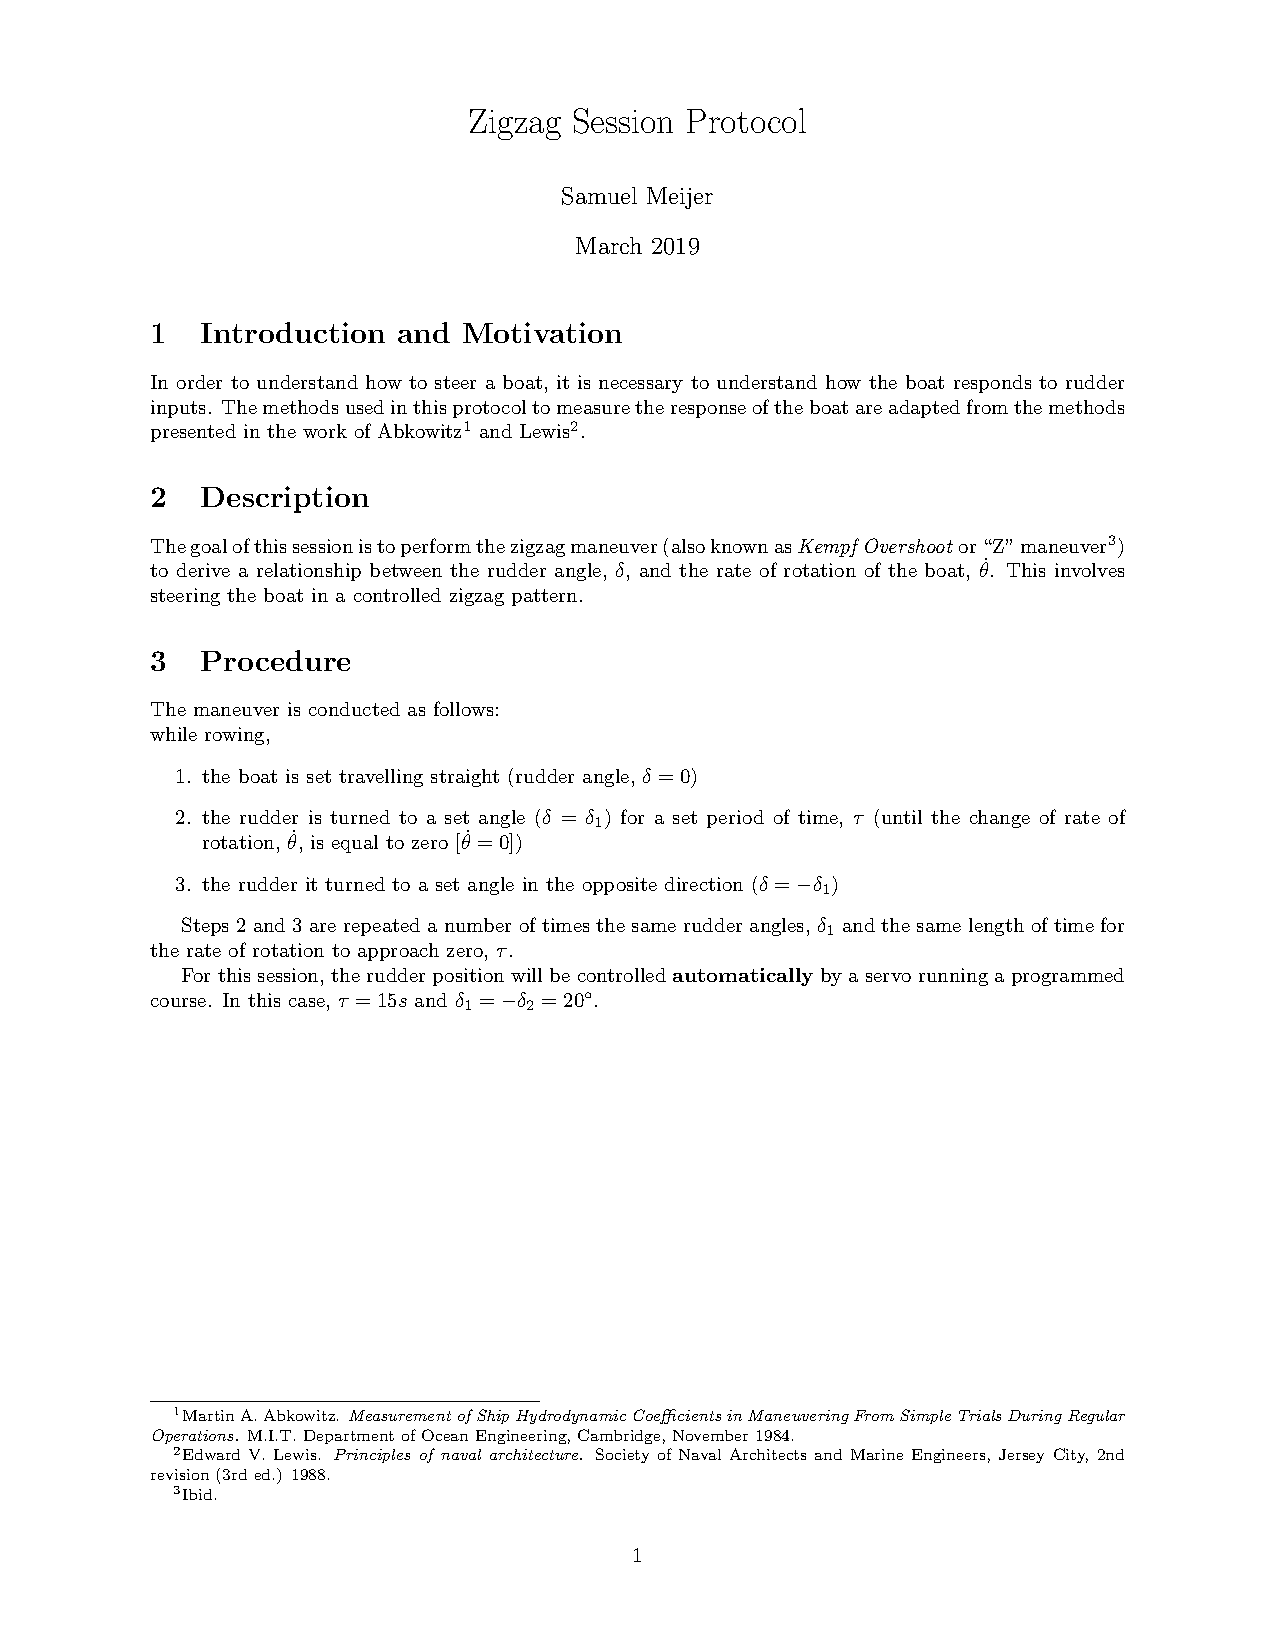
\includepdf[]{appendices/Session_Protocol-3.pdf}


% \chapter{Software}\label{app:software}
 %% You may want to include some code in your thesis. I found this method online, and would recommend you do the same... See preamble/arduinoLanguage.tex for the file that makes it look nice.
\begin{lstlisting}[language=Arduino]  
#include <Wire.h>
#include <Adafruit_Sensor.h>
#include <Adafruit_BNO055.h>
#include <utility/imumaths.h>
#include <Adafruit_GPS.h>
#include <SPI.h>
#include <SD.h>
#include <Servo.h>
#include <math.h>
#include "Filter.h"

/* This driver reads raw data from the BNO055, Potentiometer and GPS

   Connections for ADALOGGER
   ===========

   Potentiometer
   _____________
   Connect one side to VCC
   Connect other to common ground
   Connect Middle to A0

   GPS
   _____________
   Connect VIN to VCC
   Connect GROUND to common ground
   Connect GPS TX to RX1 (D0)
   Connect GPS RX to TX1 (D1)

*/

/*********************************************/
/*BNO055 (orientation) setup, variables and def'n*/
/*********************************************/
// Sample delay
const float SAMPLERATE = 10;
// Setup for the differentiation variables
double psierror = 0;
double dt = 0;
double dpsierror_dt = 0;
double previouspsierror = 0;

\end{lstlisting}

%%%%%%%%%%%%%%%%%%%%%%%%%%%%%%%%%%%%%%%%%%%
% Bibliography
%%%%%%%%%%%%%%%%%%%%%%%%%%%%%%%%%%%%%%%%%%%

\bibliographystyle{unsrt}
\bibliography{reference_files/references}{}


\end{document}